% !TeX program = xelatex 
\documentclass{zjureport}
\bibliographystyle{plain}
\usepackage{subfigure}
% =============================================
% Part 0 Edit the info
% =============================================

\major{电子信息工程}
\name{许嘉明}
\stuid{3210432040}
\college{信息科学与工程学院}
\date{\zhtoday}
\lab{Sl503}
\course{信号与系统分析}
\instructor{王一刚}
\grades{59}
\expname{课程实验报告}
\exptype{设计实验}
\partner{nil}
\class{电信212}

\begin{document}
% =============================================
% Part 1 Header
% =============================================
\makecover
\makeheader

% =============================================
% Part 2 Main document
% =============================================
\section{实验目的}
	申请GITHUB账号,并建立博客仓库。
\section{实验过程}
	\subsection{购买加速器服务}
	如果不挂加速器,网页大概率会打不开.
		\begin{figure}[!htbp]
			\centering
			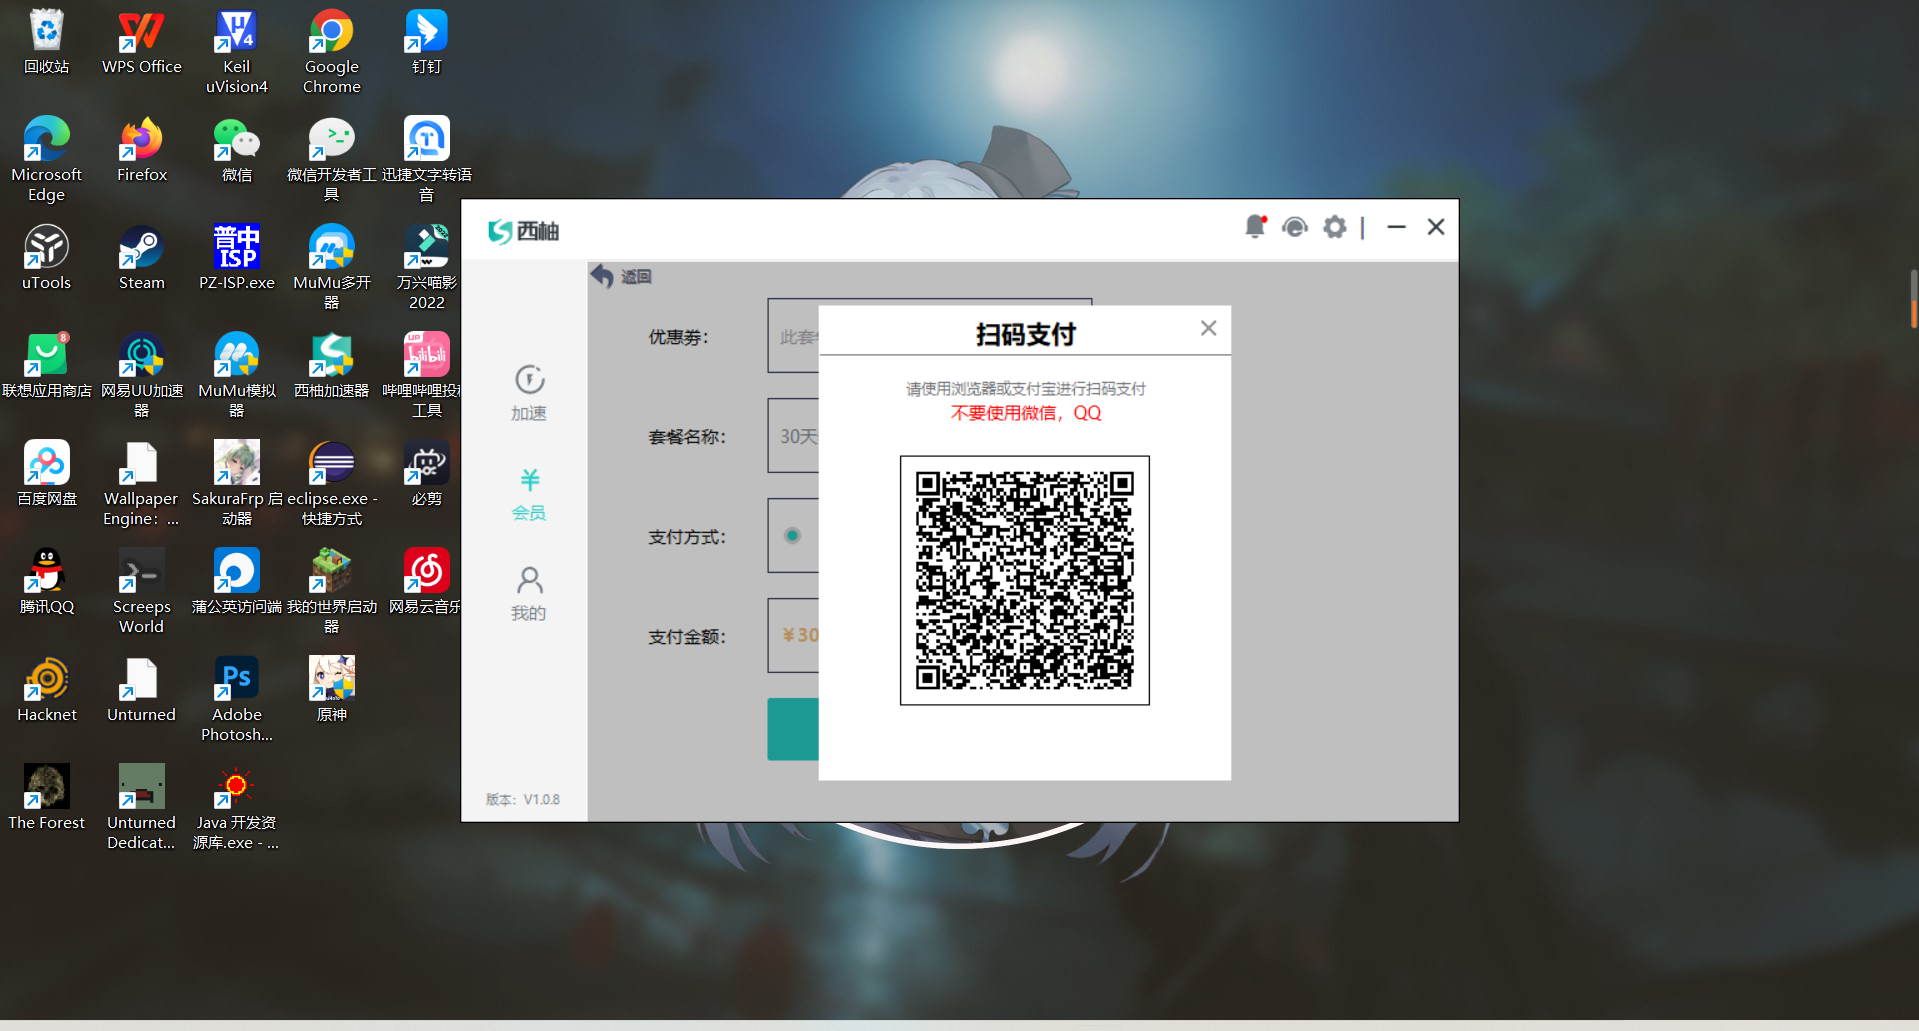
\includegraphics[width=0.6\linewidth]{1.png}
			\caption{VPN服务}
			\label{fig:dist}
		\end{figure}
	\subsection{申请Github账号}
		\begin{enumerate}
			\item{通过网址:https://github.com 进入Github主页,进入主页后可通过qq邮箱等注册一个Github账号,具体操作步骤请根据引导进行即可}(详情请看图3至图6)
		\end{enumerate}
\begin{figure}[htbp]
	\centering
	\subfigure{
		\begin{minipage}{4.5cm}
			\centering
			
\includegraphics[width=5cm]{web1.png}
			\caption{主页}
		\end{minipage}%
	}%
	\subfigure{
		\begin{minipage}{7cm}
			\centering
			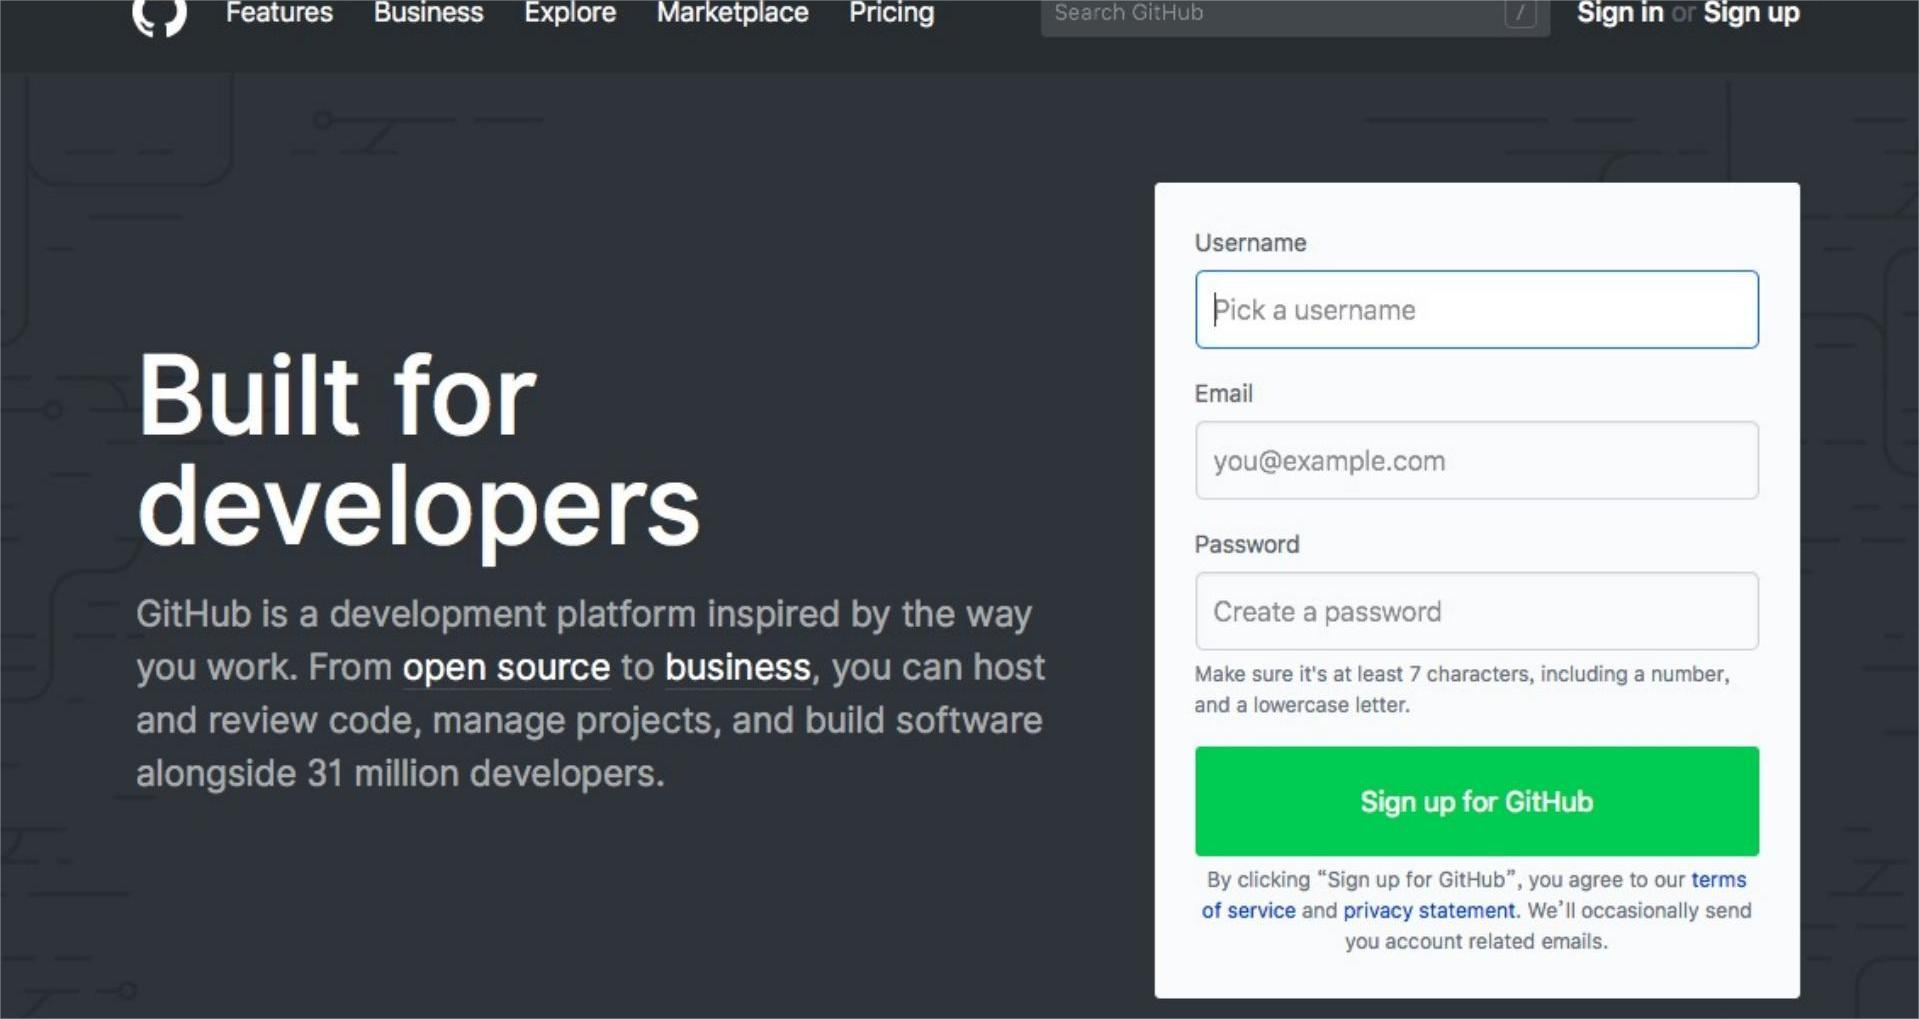
\includegraphics[width=5cm]{web2.png}
			\caption{注册页}
		\end{minipage}
	}
	\subfigure{
		\begin{minipage}{4.5cm}
			\centering
			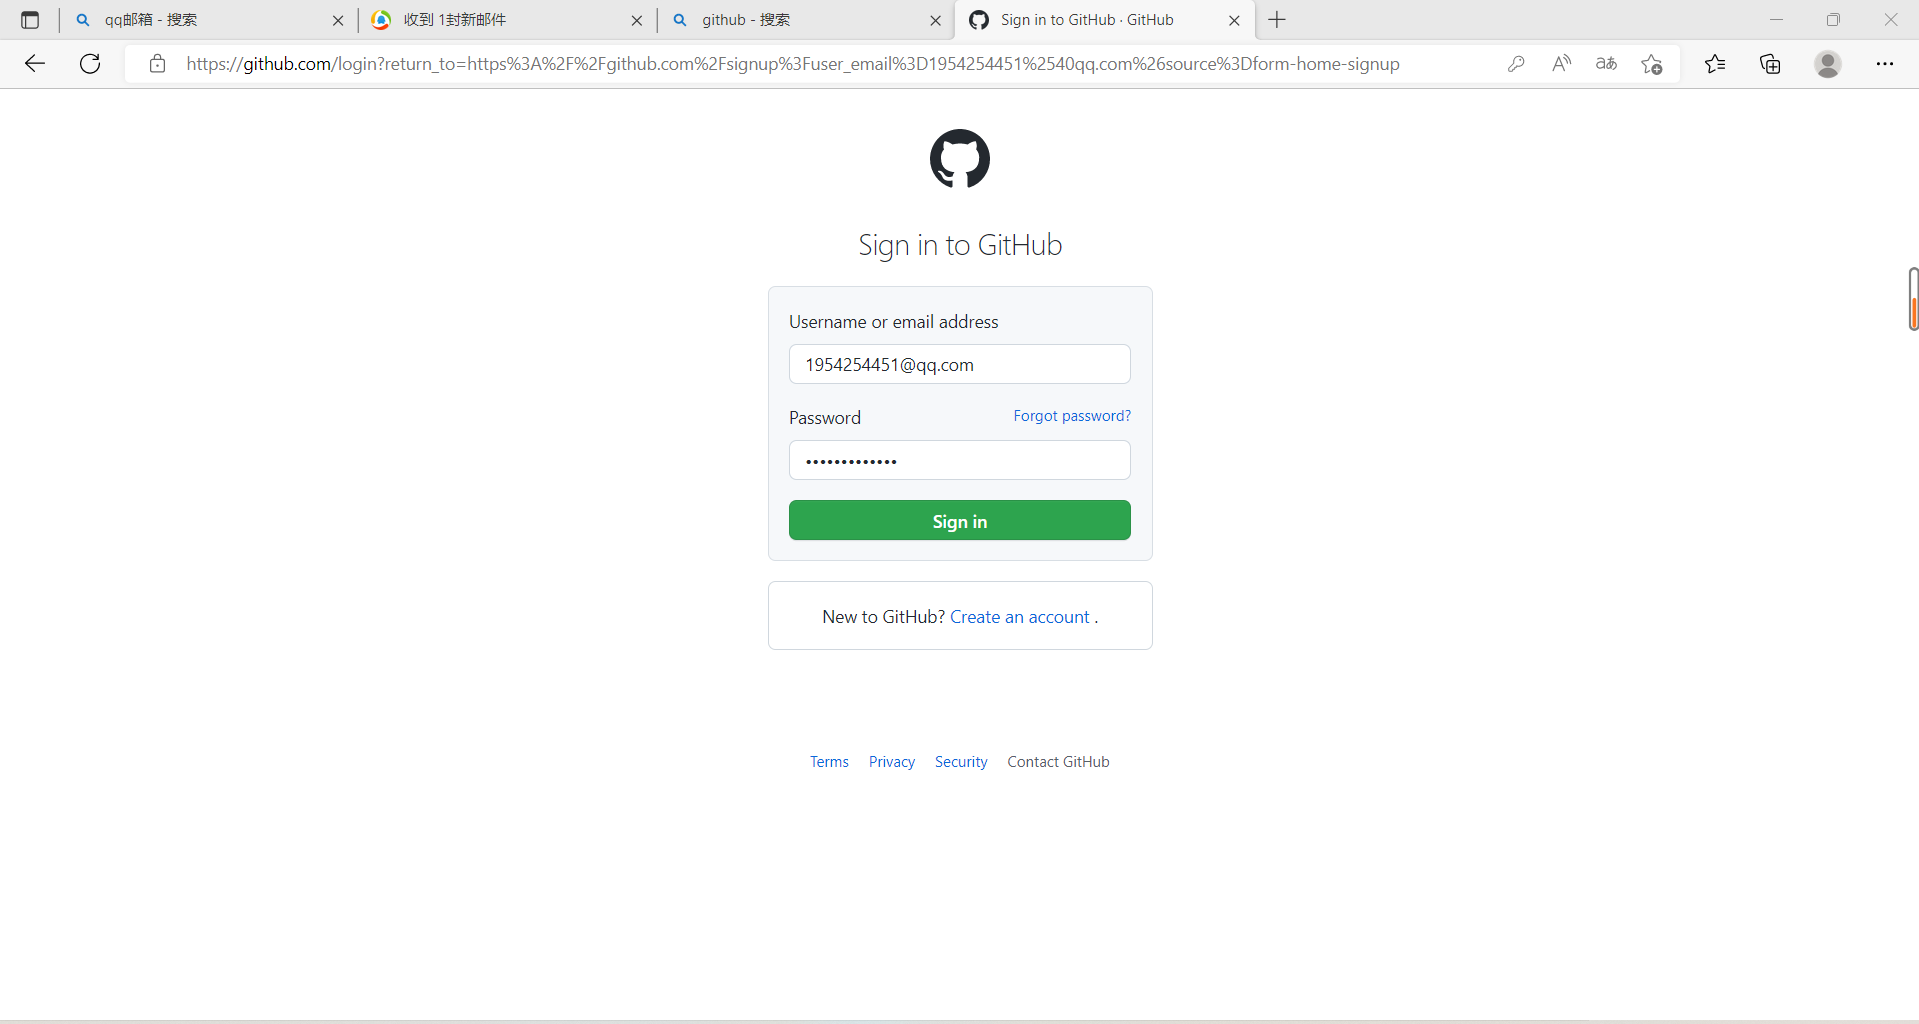
\includegraphics[width=5cm]{web3.png}
			\caption{登录页}
		\end{minipage}%
	}%
	\subfigure{
		\begin{minipage}{7cm}
			\centering
			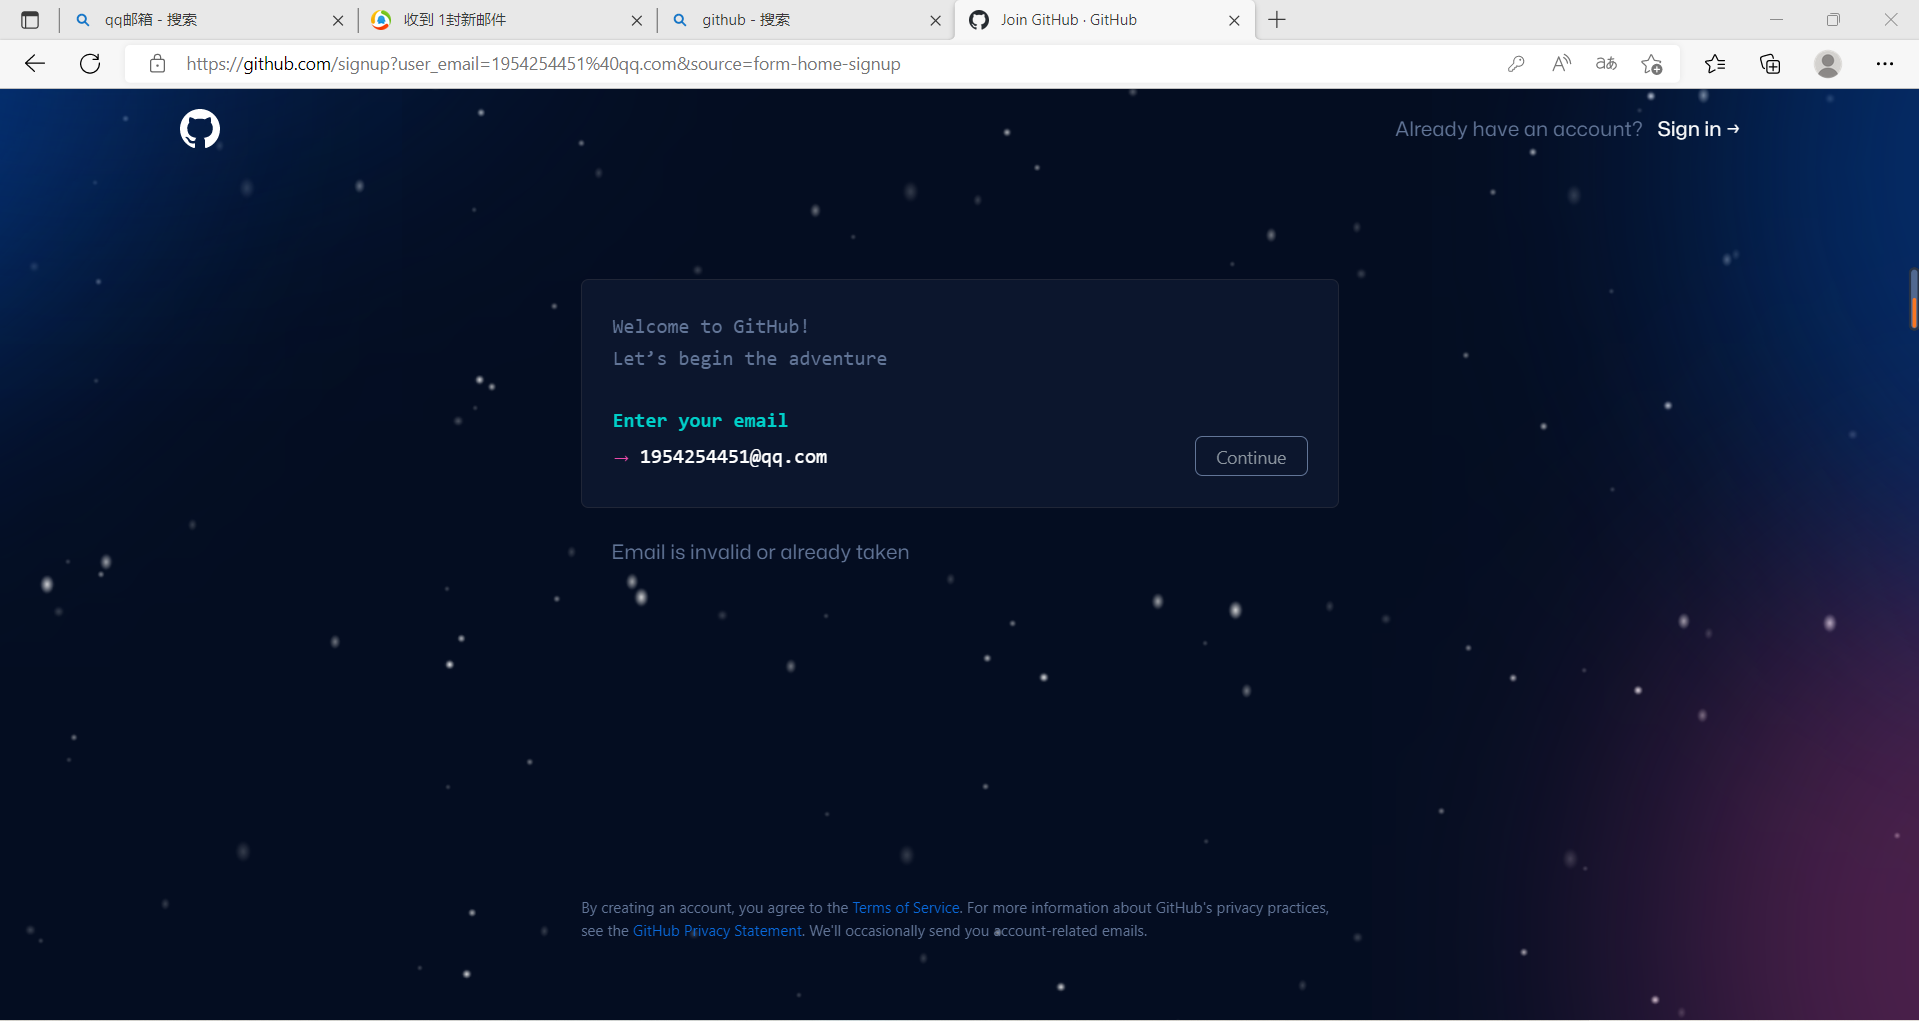
\includegraphics[width=5cm]{web4.png}
			\caption{登录页}
		\end{minipage}
	}
\end{figure}
	
	
	
	\subsection{安装并配置Git}
	\begin{enumerate}
		\item 由于sudo是linux的系统管理指令,而本人用的是windows操作系统,所以选择在官网下载安装(https://git-scm.com/download/win)
		\lstinputlisting[language=MATLAB]{code/command1.m}
		\item{打开Git Bash命令行输入对应配置命令,配置用户信息,如下图所示:}
		\lstinputlisting[language=MATLAB]{code/command2.m}
		\begin{figure}[!htbp]
			\centering
			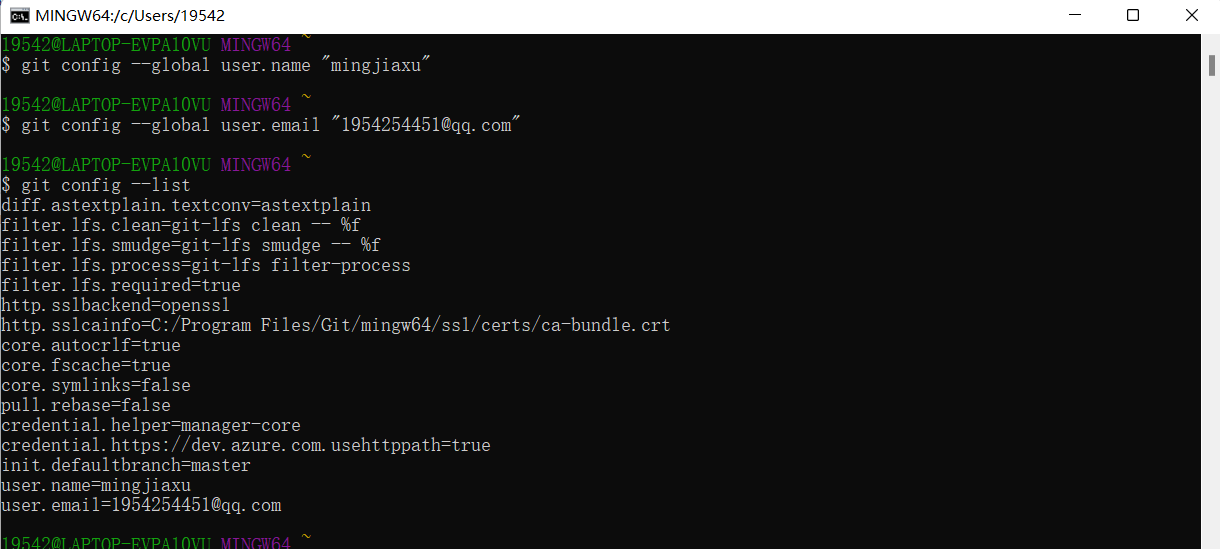
\includegraphics[width=0.6\linewidth]{pezhi.png}
			\caption{配置用户信息}
			\label{fig:dist}
		\end{figure}
	\end{enumerate}
	\subsection{安装ssh并于Github添加公钥}
		\begin{enumerate}
			\item{下载安装ssh}与安装Git时情况相同,我们无法直接使用sudo命令直接下载ssh,同样的,我选择了在官网下载,我选择的是OpenSSH-Win64.zip(https://github.com/PowerShell/Win32-OpenSSH/releases ),如下图所示
			\lstinputlisting[language=MATLAB]{code/command3.m}
			\begin{figure}[!htbp]
				\centering
				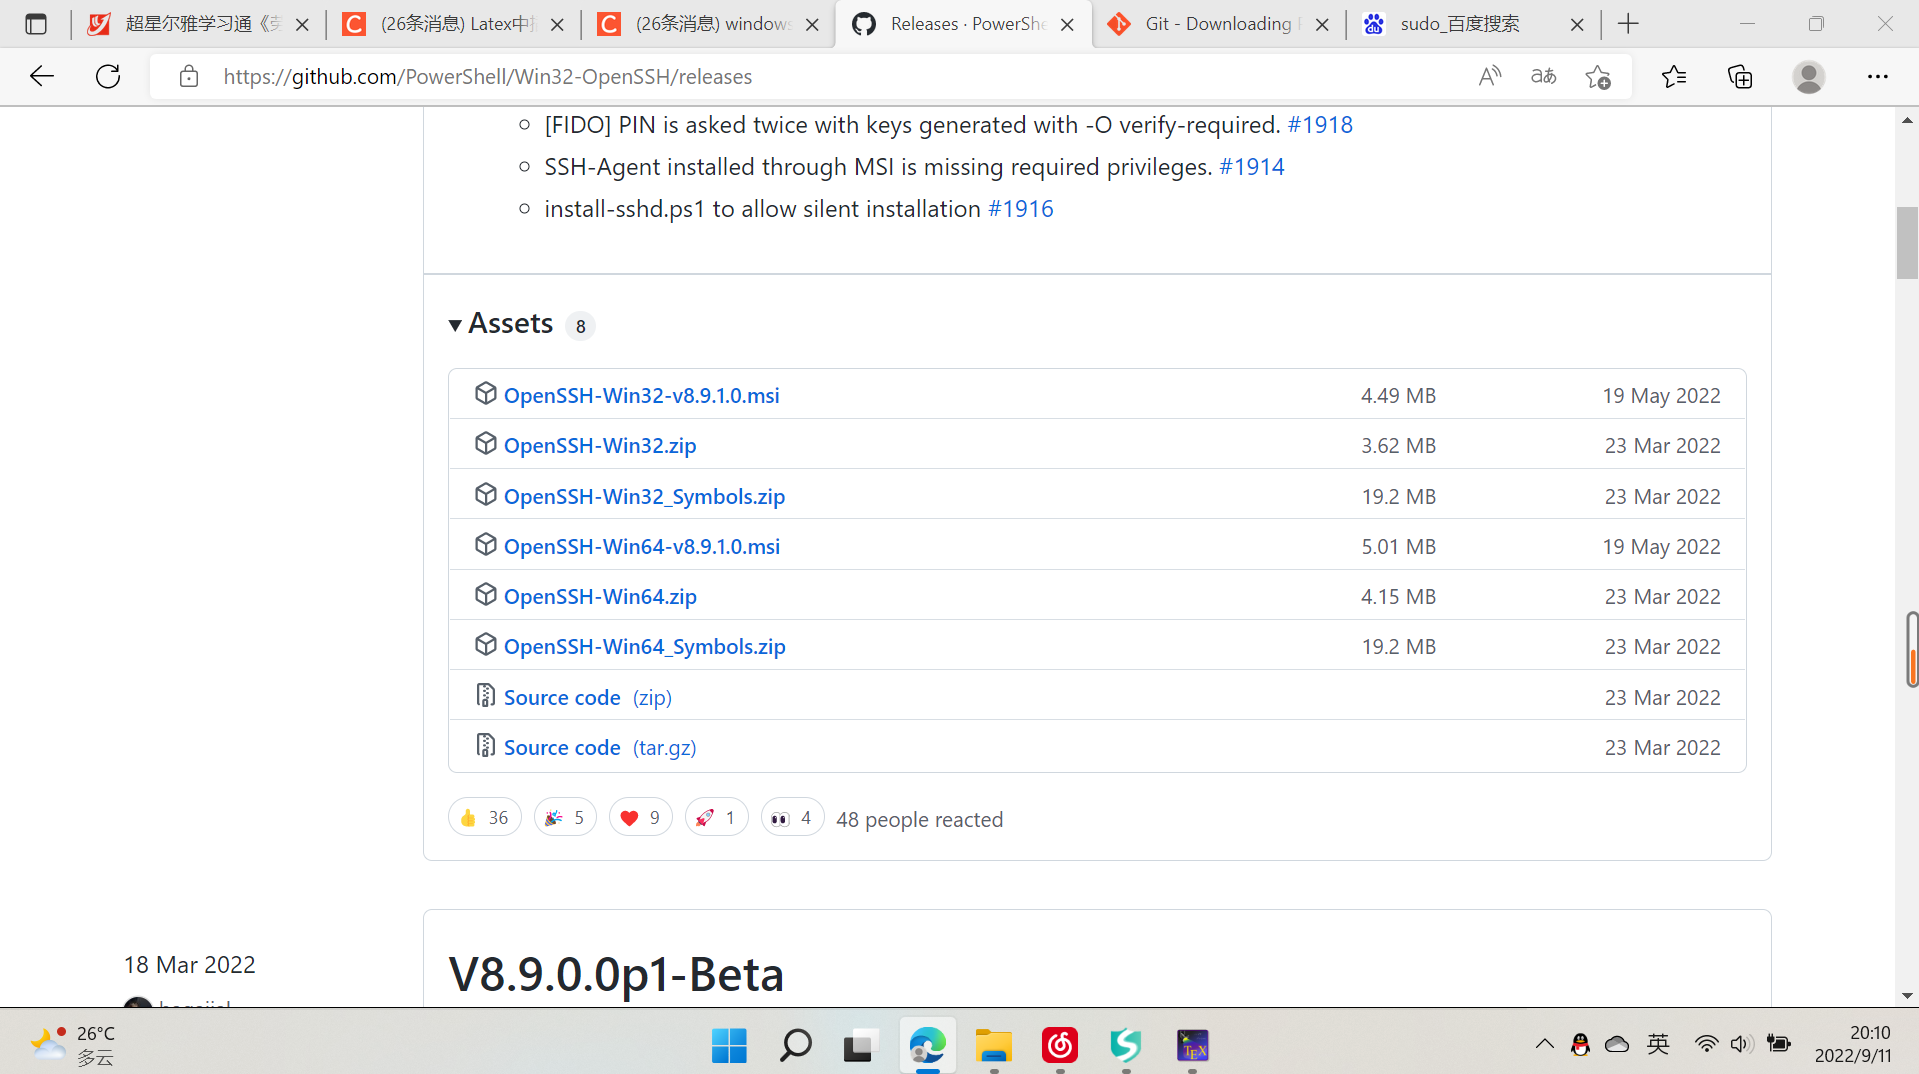
\includegraphics[width=0.6\linewidth]{ssh.png}
				\caption{ssh下载页面}
				\label{fig:dist}
			\end{figure}
			\item{创建密钥文件}win+r打开cmd,输入以下指令,啥都不用填,直接回车过。
			\lstinputlisting[language=MATLAB]{code/command4.m}
		
			\item{将公钥添加到Github}
				\subitem{查看生成公钥}
					找到.ssh文件夹(文件路径基本都一样,只是名字不同)
					在如图所示位置输入cmd打开命令行,输入以下指令查看公钥,直接打开$id_rsa$文件可能打不开
					
					\lstinputlisting[language=MATLAB]{code/command5.m}
					
					\begin{figure}[htbp]
					\centering
					\subfigure{
						\begin{minipage}{4.5cm}
							\centering
							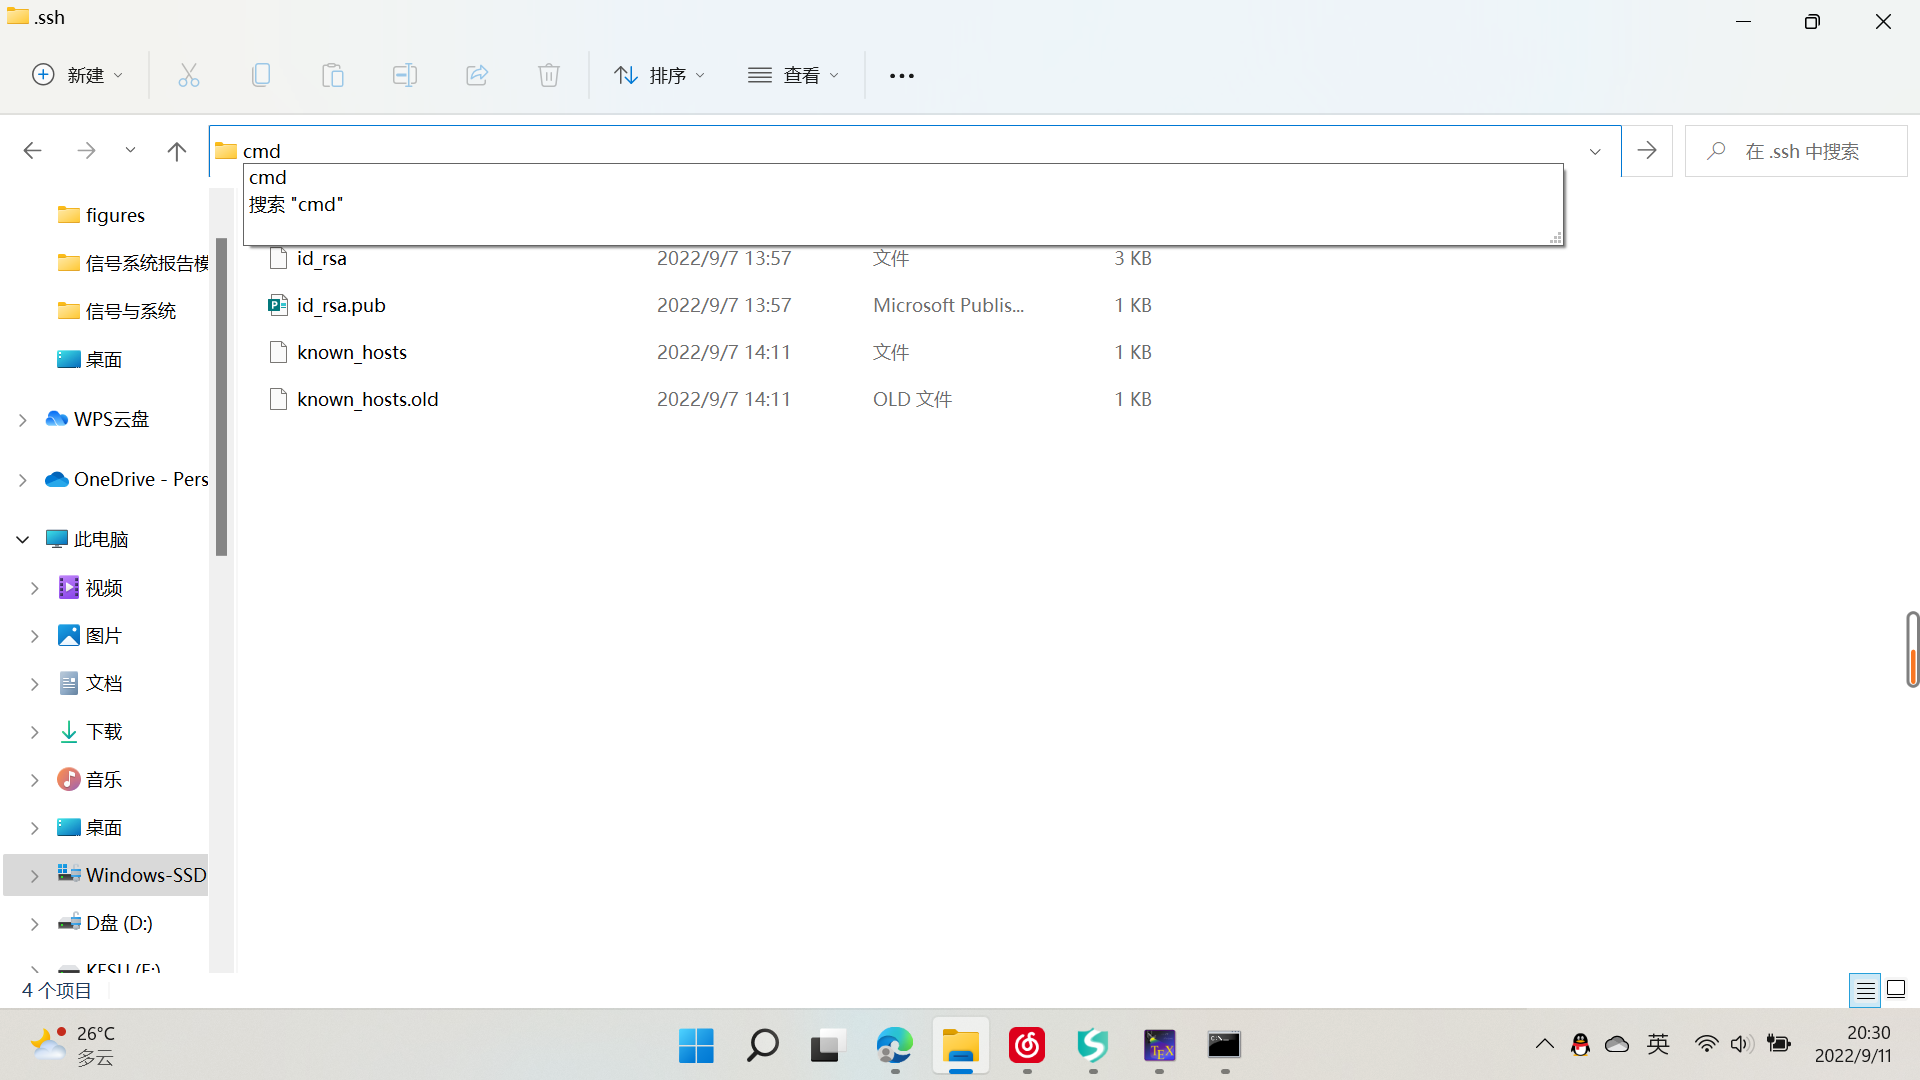
\includegraphics[width=5cm]{cmd2.png}
							\caption{命令行打开位置}
						\end{minipage}
					}
					\subfigure{
						\begin{minipage}{7cm}
							\centering
							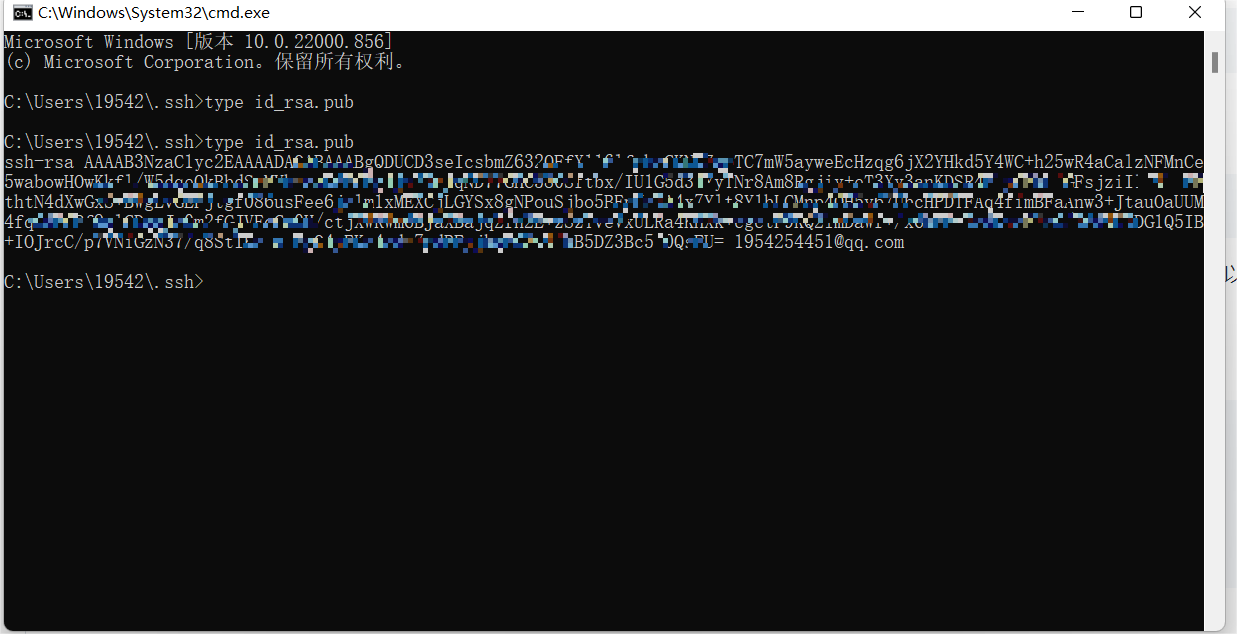
\includegraphics[width=5cm]{cmd3.png}
							\caption{命令行指令输入}
						\end{minipage}
					}
				\end{figure}
				\subitem{添加公钥至Github}
				\begin{figure}[htbp]
					\centering
					\subfigure{
						\begin{minipage}{4.5cm}
							\centering
							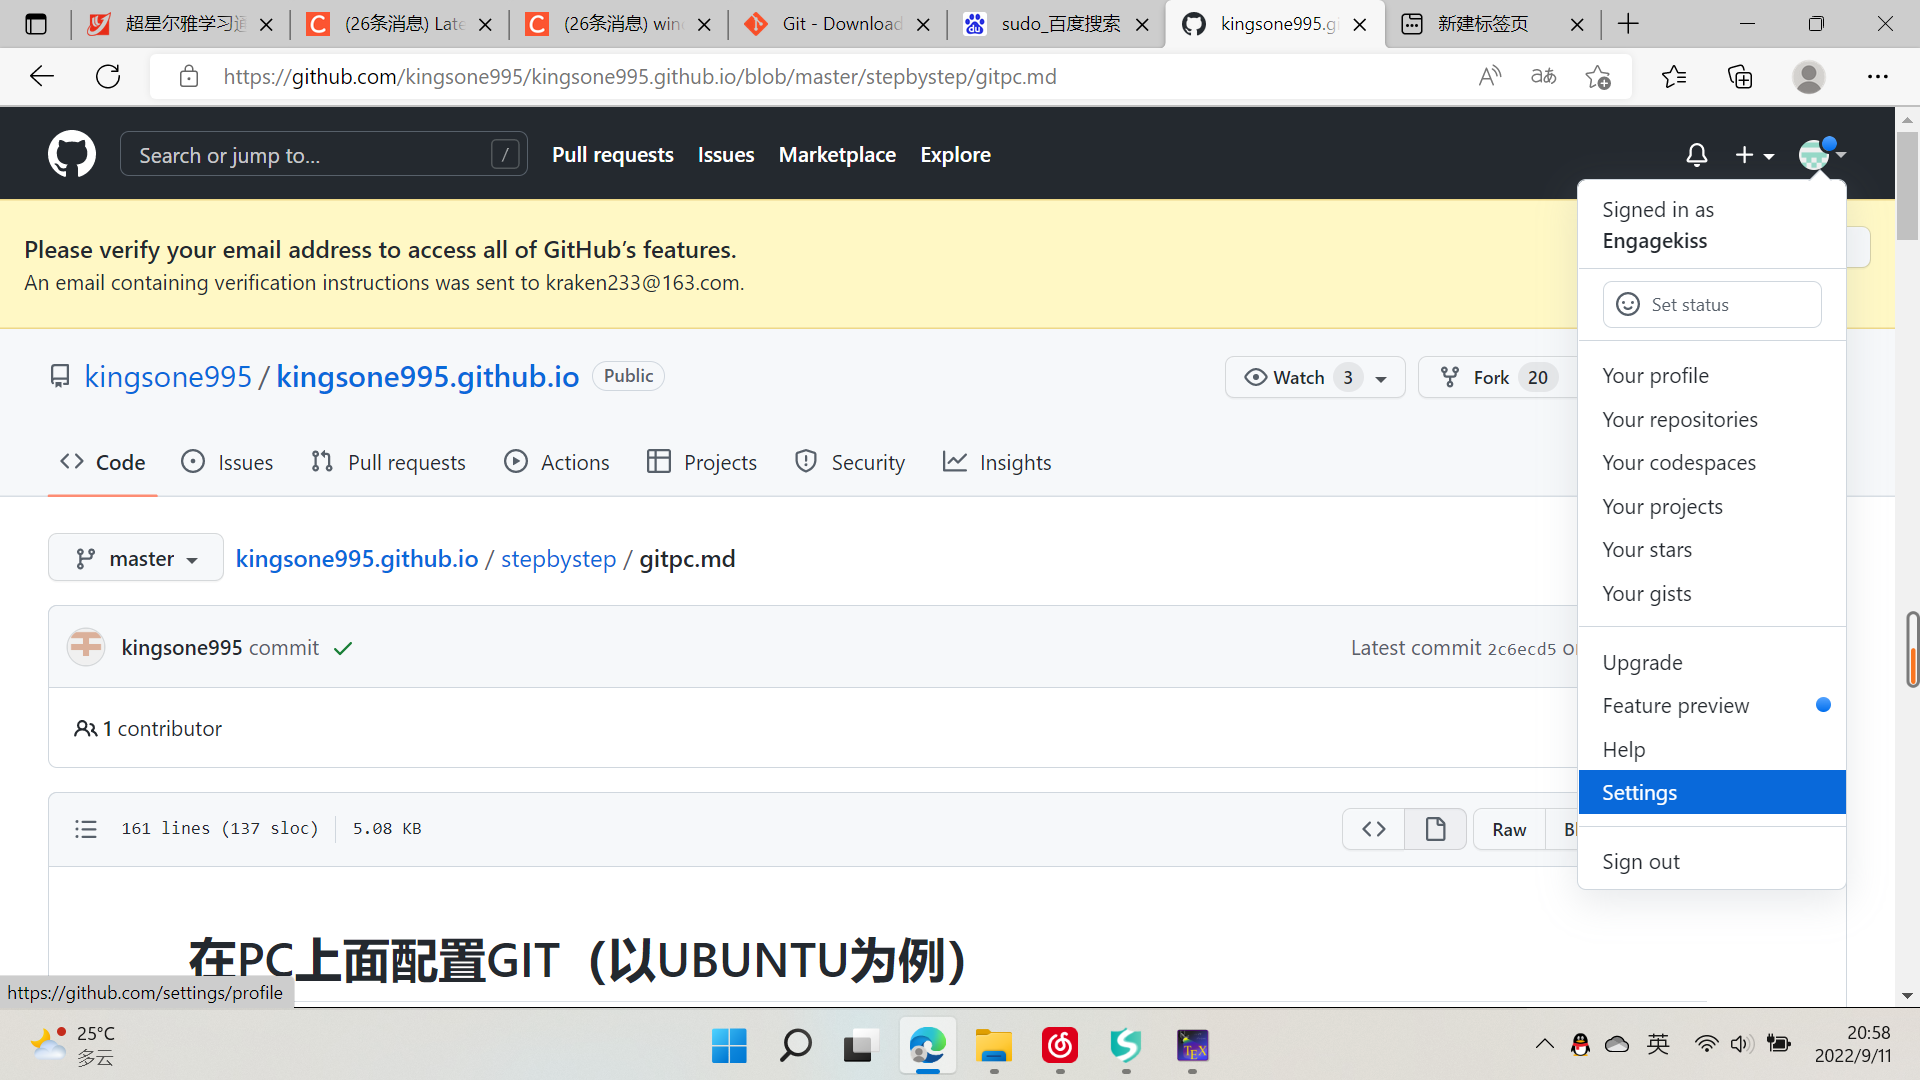
\includegraphics[width=5cm]{tianjia (1).png}
						\end{minipage}%
					}%
					\subfigure{
						\begin{minipage}{7cm}
							\centering
							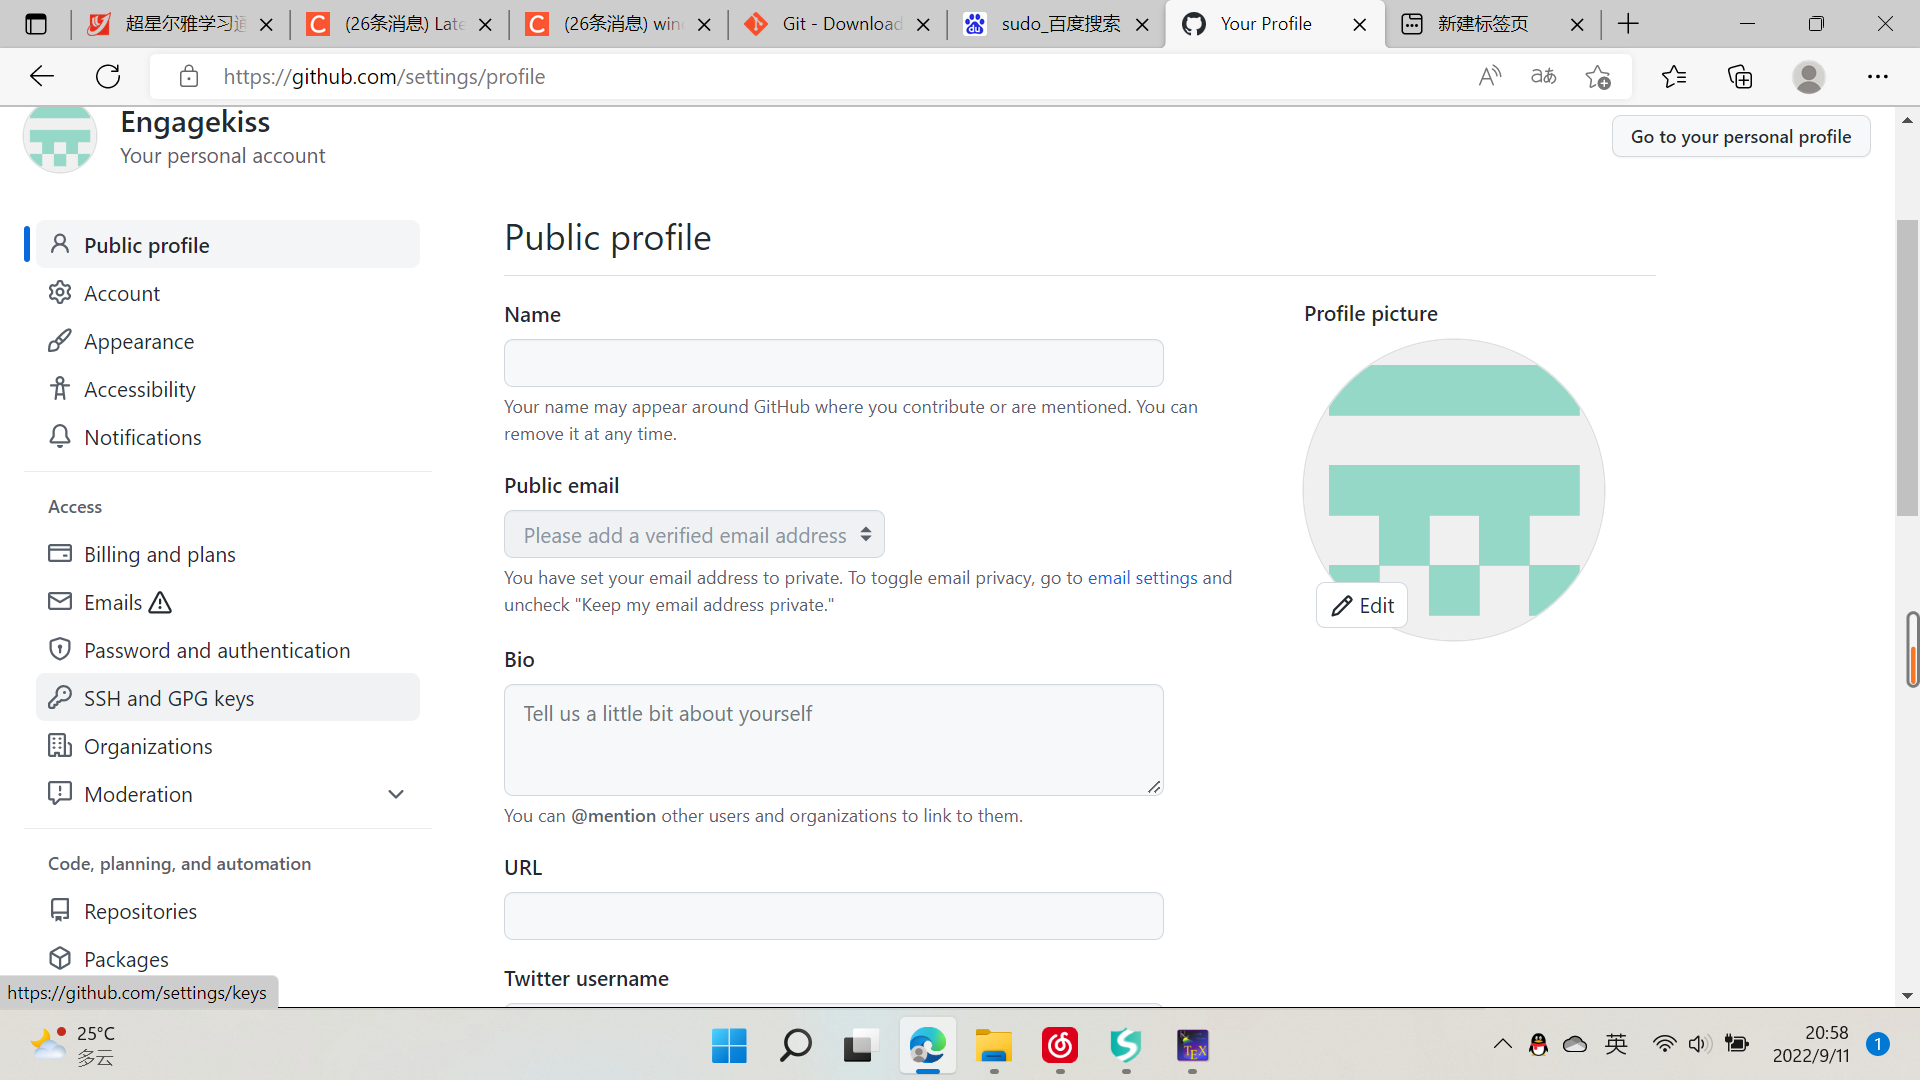
\includegraphics[width=5cm]{tianjia (2).png}
						\end{minipage}
					}
					\subfigure{
						\begin{minipage}{4.5cm}
							\centering
							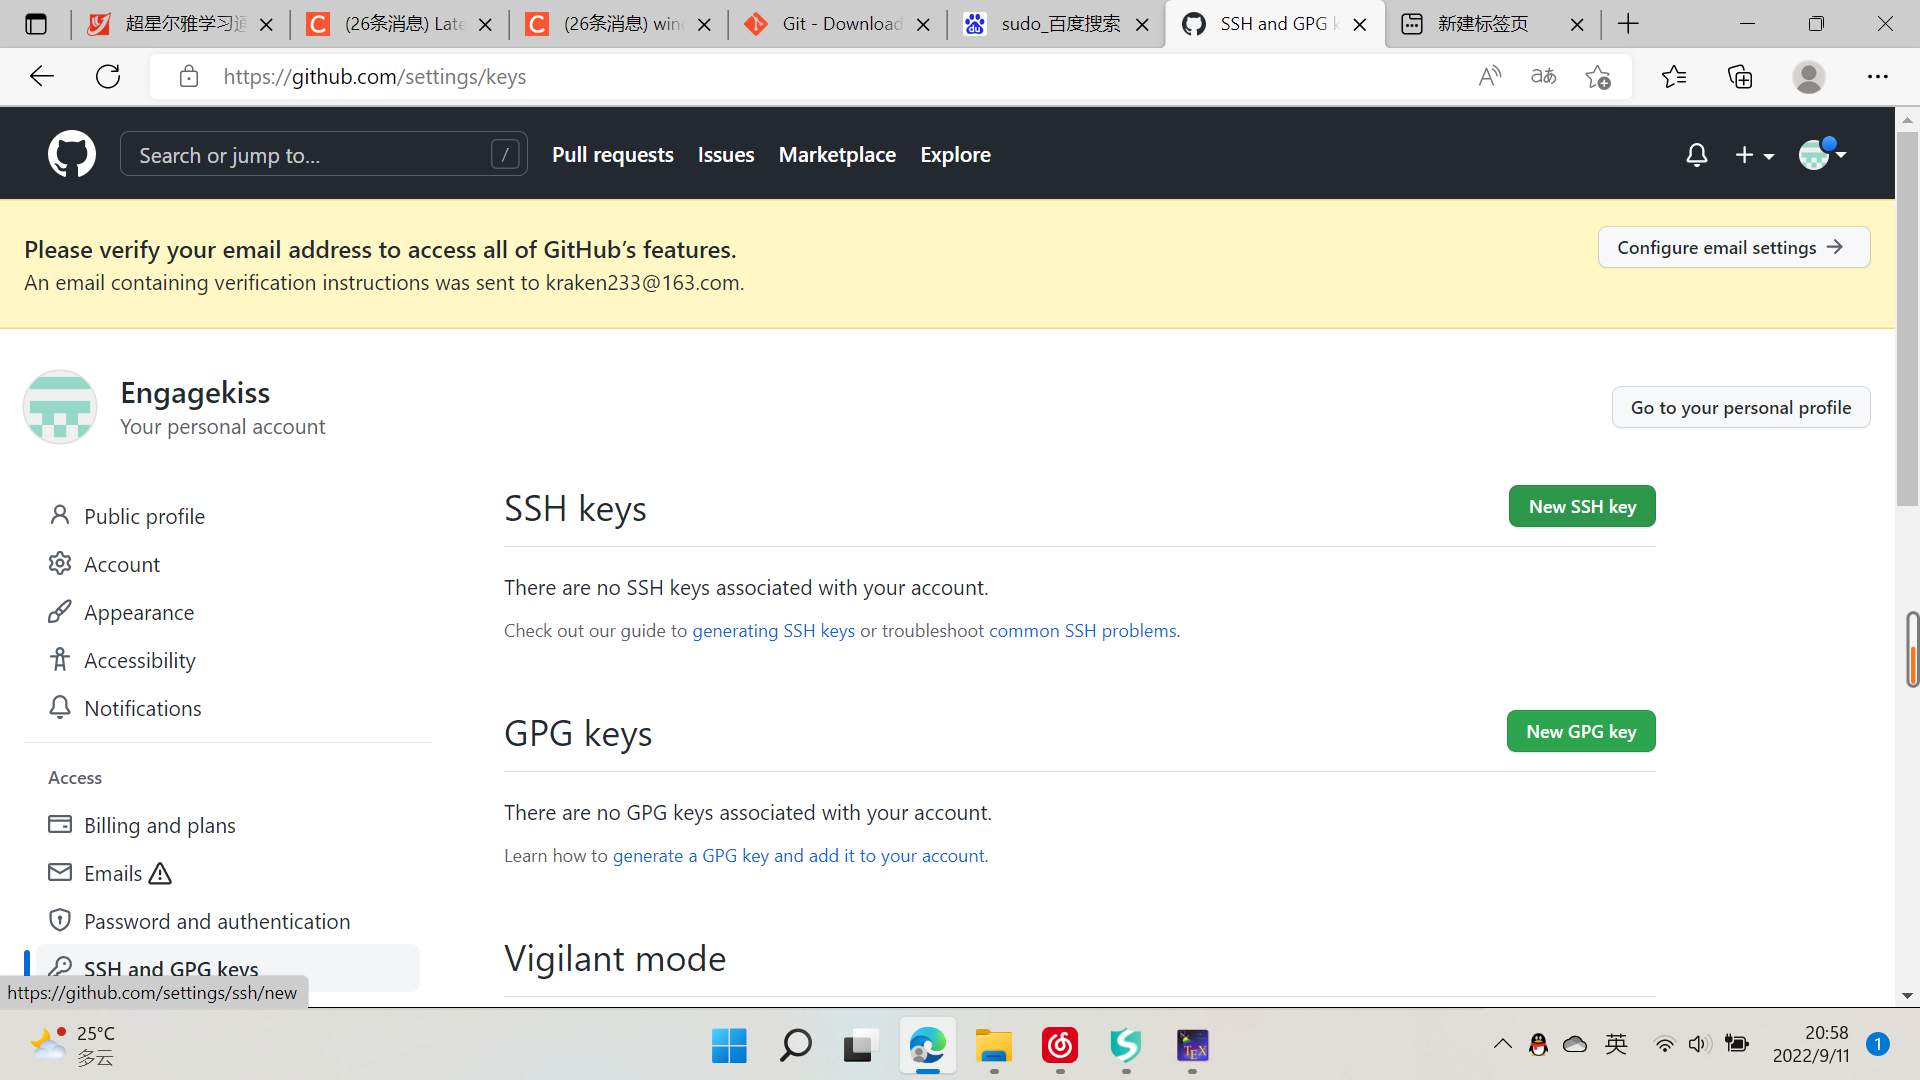
\includegraphics[width=5cm]{tianjia (3).png}
						\end{minipage}%
					}%
					\subfigure{
						\begin{minipage}{7cm}
							\centering
							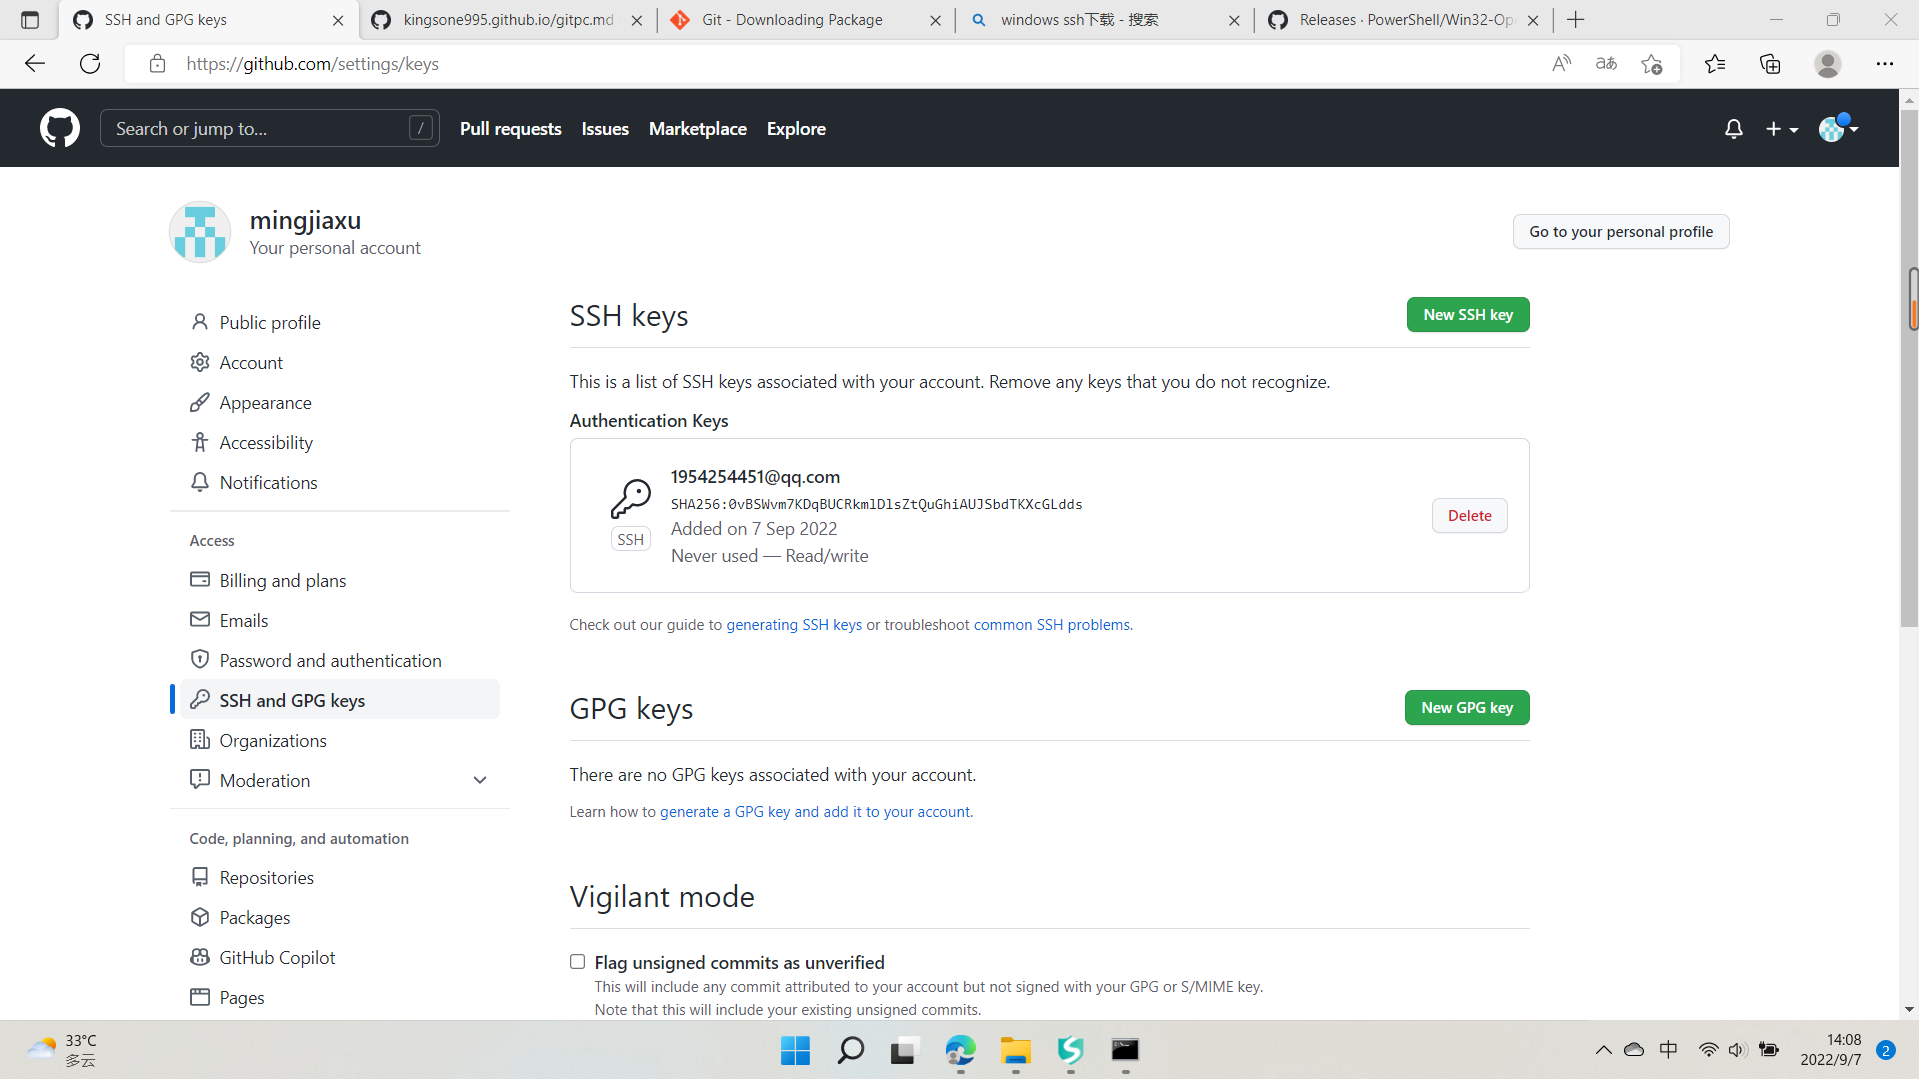
\includegraphics[width=5cm]{tianjia (4).png}
						\end{minipage}
					}
				\end{figure}
		\end{enumerate}
	\subsection{创建博客仓库并进行功能测试}
	
	
\section{实验内容}


\end{document}
